\documentclass[border=20pt]{standalone}
\usepackage{tikz}
\usepackage{graphicx}
\usetikzlibrary{shapes.geometric, arrows.meta, positioning, fit, backgrounds, calc}

\begin{document}
\begin{tikzpicture}[
    auto,
    font=\sffamily\Large,
    % Styles definition
    base/.style = {draw, align=center, inner sep=1.8ex, rounded corners=3pt, minimum width=4.5cm},
    input/.style = {base, fill=gray!20, font=\sffamily\huge\bfseries},
    process/.style = {base, fill=white, font=\sffamily\Large\bfseries, text=black},
    decision/.style = {draw, diamond, aspect=1.4, fill=purple!10, text width=3.5cm, align=center, inner sep=0.5ex, font=\sffamily\Large\bfseries, text=black},
    output/.style = {base, fill=gray!20, font=\sffamily\huge\bfseries, text width=6cm, minimum height=2.5cm},
    arrow/.style = {-{Latex[scale=1.2]}, thick, draw=black!70},
    % Module containers (dashed boundary matching the reference image style)
    mod_container/.style = {draw, dashed, thick, rounded corners=5pt, inner xsep=15pt, inner ysep=15pt},
    modtitle/.style = {font=\sffamily\huge\bfseries, align=center}
]

% ====================
% COLUMN 1: Input Layer
% ====================
\node [input, fill=white] (vid) {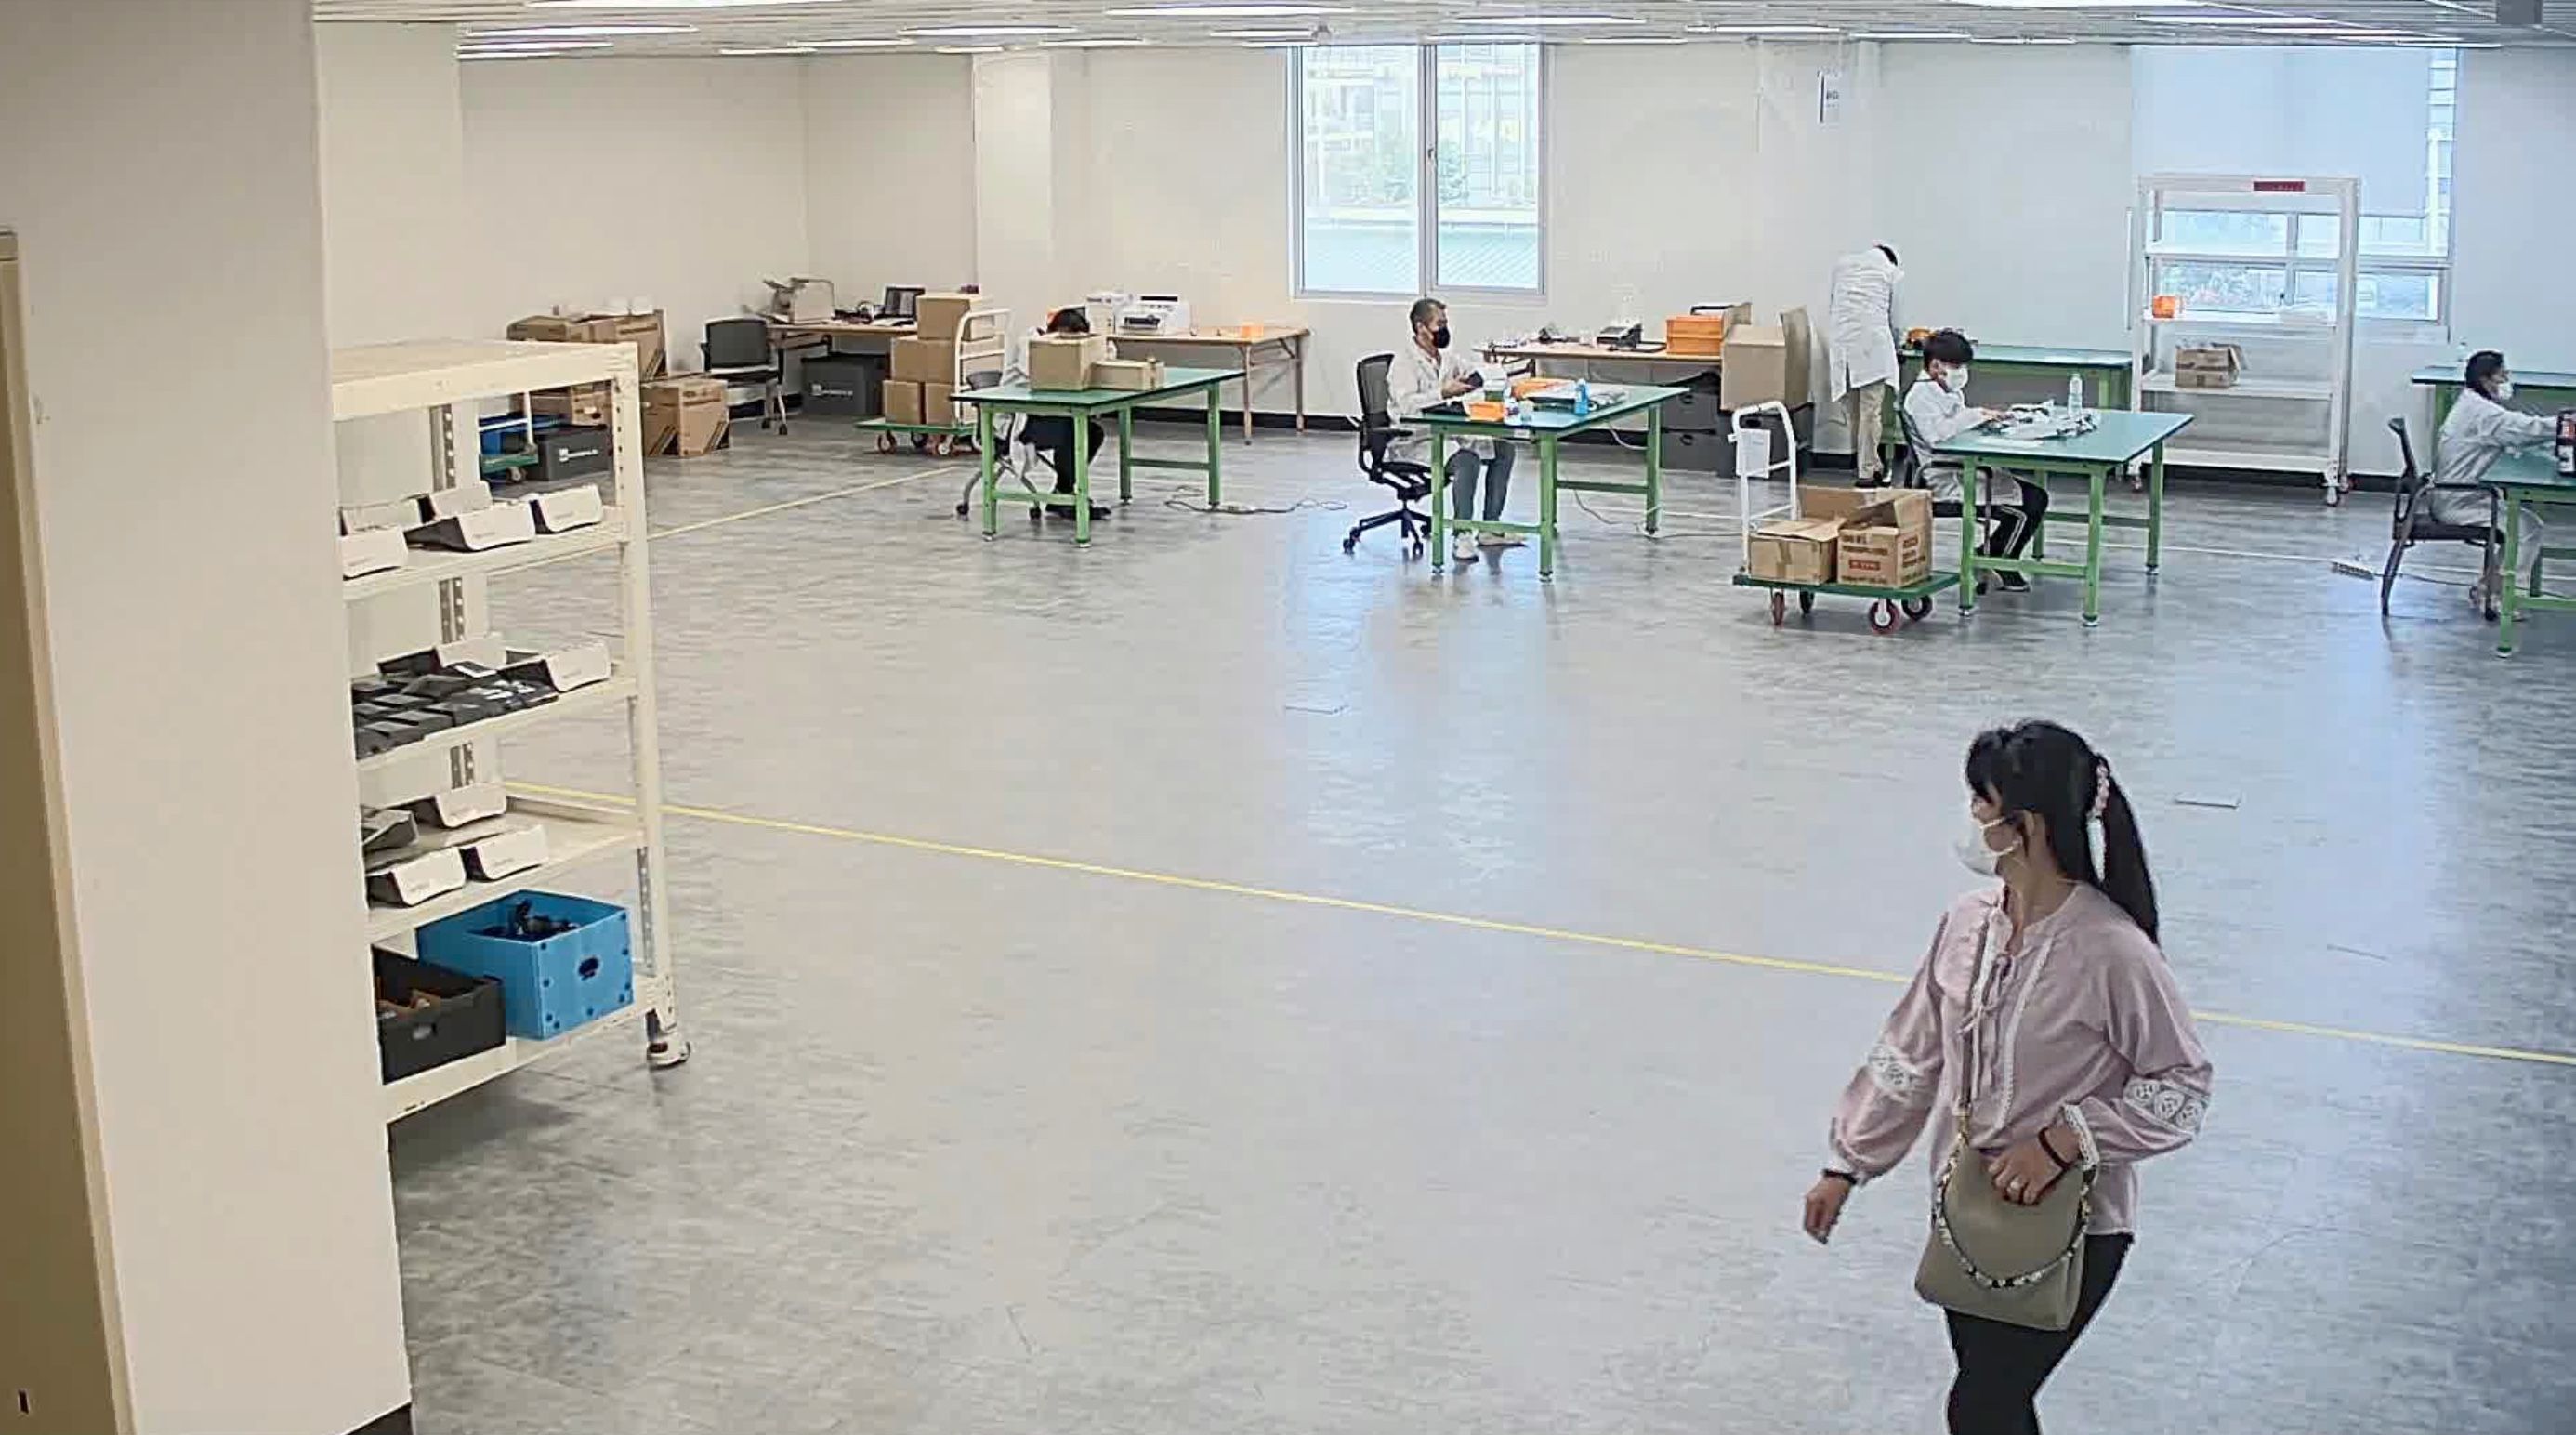
\includegraphics[width=3cm]{input_frame.jpeg}\\[1ex]Video Frames};
\node [process, below=0.8cm of vid] (norm) {Resizing \& Norm\\($480 \times 480 \times 3$)};
\draw [arrow] (vid) -- (norm);

\begin{scope}[on background layer]
    \node[draw=gray!50, fill=gray!5, mod_container, fit=(vid)(norm)] (input_layer) {};
    \node[modtitle, text=black!80, above=5pt of input_layer] {Input Layer};
\end{scope}

% ====================
% COLUMN 2: YOLO
% ====================
\node [process, right=3.5cm of input_layer.east, yshift=1.5cm] (m1_1) {CNN Backbone};
\node [process, below=0.6cm of m1_1] (m1_2) {NMS-Free\\Decoupled Head};
\node [process, below=0.6cm of m1_2] (m1_3) {Confidence\\Thr $> 0.3$};
\node [process, below=0.6cm of m1_3, fill=white, inner sep=1ex] (m1_4) {Output: BBox\\Coordinates\\[1ex]
    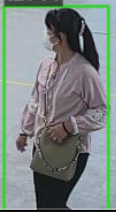
\includegraphics[height=1.1cm]{bbox1.png} 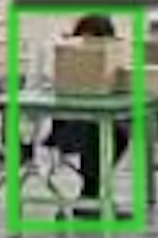
\includegraphics[height=1.1cm]{bbox2.png} 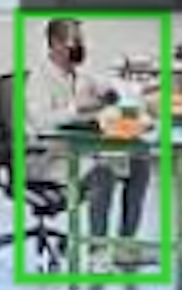
\includegraphics[height=1.1cm]{bbox3.png}\\[2pt]
    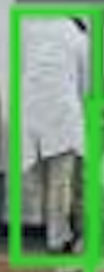
\includegraphics[height=1.1cm]{bbox4.png} 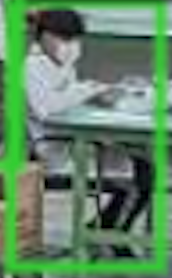
\includegraphics[height=1.1cm]{bbox5.png} 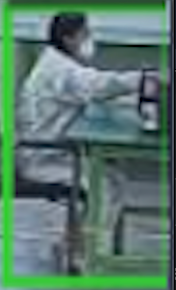
\includegraphics[height=1.1cm]{bbox6.png}
};

\draw [arrow] (m1_1) -- (m1_2);
\draw [arrow] (m1_2) -- (m1_3);
\draw [arrow] (m1_3) -- (m1_4);

\begin{scope}[on background layer]
    \node[draw=red!50, fill=red!5, mod_container, fit=(m1_1)(m1_4)] (mod1) {};
    \node[modtitle, text=red!50!black, above=5pt of mod1] {Module 1: Detection\\{[}YOLOv26m{]}};
\end{scope}

\draw [arrow] (input_layer.east |- mod1.west) -- (mod1.west);

% ====================
% COLUMN 3: ByteTrack
% ====================
\node [process, right=5cm of m1_1] (m2_1) {Kalman Filter};
\node [process, below=0.6cm of m2_1] (m2_2) {Two-Round\\IoU Matching};
\node [process, below=0.6cm of m2_2] (m2_3) {20-Frame\\Track Buffer};
\node [process, below=0.6cm of m2_3, fill=white, inner sep=1ex] (m2_4) {Output: Local Track IDs\\[1ex]
    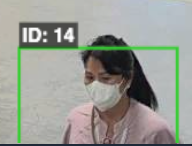
\includegraphics[height=1.1cm]{track1.png} 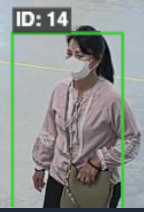
\includegraphics[height=1.1cm]{track2.png} 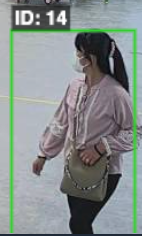
\includegraphics[height=1.1cm]{track3.png}
};

\draw [arrow] (m2_1) -- (m2_2);
\draw [arrow] (m2_2) -- (m2_3);
\draw [arrow] (m2_3) -- (m2_4);

\begin{scope}[on background layer]
    \node[draw=green!60!black, fill=green!5, mod_container, fit=(m2_1)(m2_4)] (mod2) {};
    \node[modtitle, text=green!50!black, above=5pt of mod2] {Module 2: Tracking\\{[}ByteTrack{]}};
\end{scope}

\draw [arrow] (mod1.east) -- (mod2.west |- mod1.east);

% ====================
% COLUMN 4: Decision Node
% ====================
\node [decision, right=2.5cm of mod2.east] (dec) {Camera views\\overlap?};
\draw [arrow] (mod2.east) -- (dec.west);

% ====================
% COLUMN 5: Modules 3 & 4 (Top & Bottom Branches)
% ====================
% Module 3 (Top)
\node [process, right=3cm of dec.east, yshift=7.5cm] (m3_1) {Extract foot\\proxy coords};
\node [process, below=0.6cm of m3_1] (m3_2) {Multiply by\\Homography (H)};
\node [process, below=0.6cm of m3_2] (m3_3) {Hungarian\\Assignment};
\node [process, below=0.6cm of m3_3, fill=white, inner sep=1ex] (m3_4) {Merge if dist.\ $< 100/200$\,px\\[1ex]
    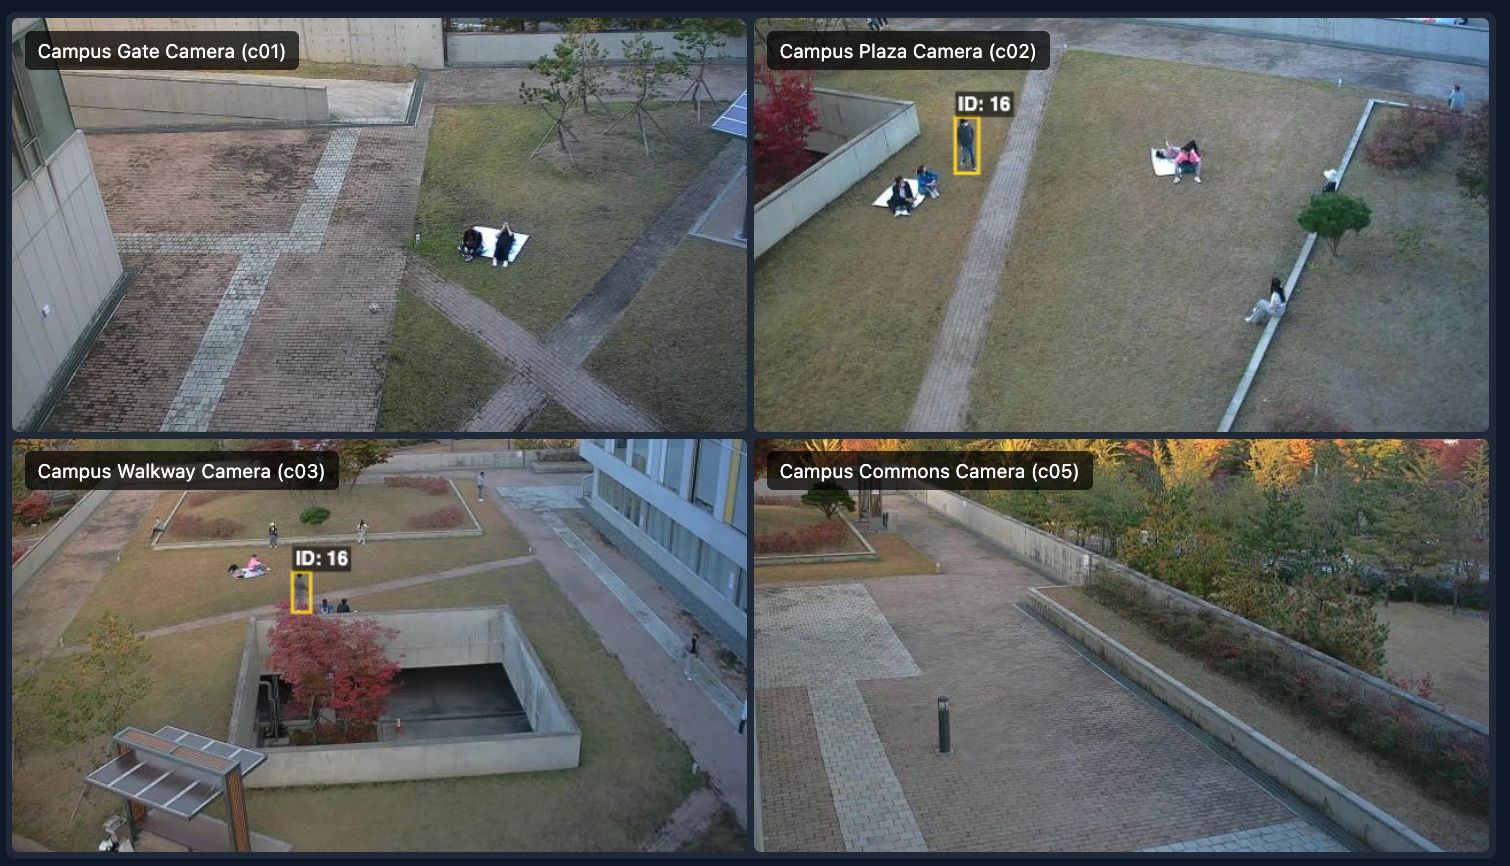
\includegraphics[height=1.6cm]{homography1.jpeg}
};

\draw [arrow] (m3_1) -- (m3_2);
\draw [arrow] (m3_2) -- (m3_3);
\draw [arrow] (m3_3) -- (m3_4);

\begin{scope}[on background layer]
    \node[draw=blue!50, fill=blue!5, mod_container, fit=(m3_1)(m3_4)] (mod3) {};
    \node[modtitle, text=blue!60!black, above=5pt of mod3] {Module 3: Mapping\\{[}Homography{]}};
\end{scope}

\draw [arrow] (dec.north) |- node[above, near start, font=\sffamily\huge\bfseries] {Yes} (mod3.west);

% Module 4 (Bottom)
\node [process, right=3cm of dec.east, yshift=-6cm] (m4_1) {Trigger: 5\%\\edge margin};
\node [process, below=0.6cm of m4_1] (m4_2) {Extract 512-dim\\embedding};
\node [process, below=0.6cm of m4_2] (m4_3) {Store in FAISS\\(60s expiry)};
\node [process, below=0.6cm of m4_3, fill=white, inner sep=1ex] (m4_4) {Match if Cosine Sim $> 0.70$\\[1ex]
    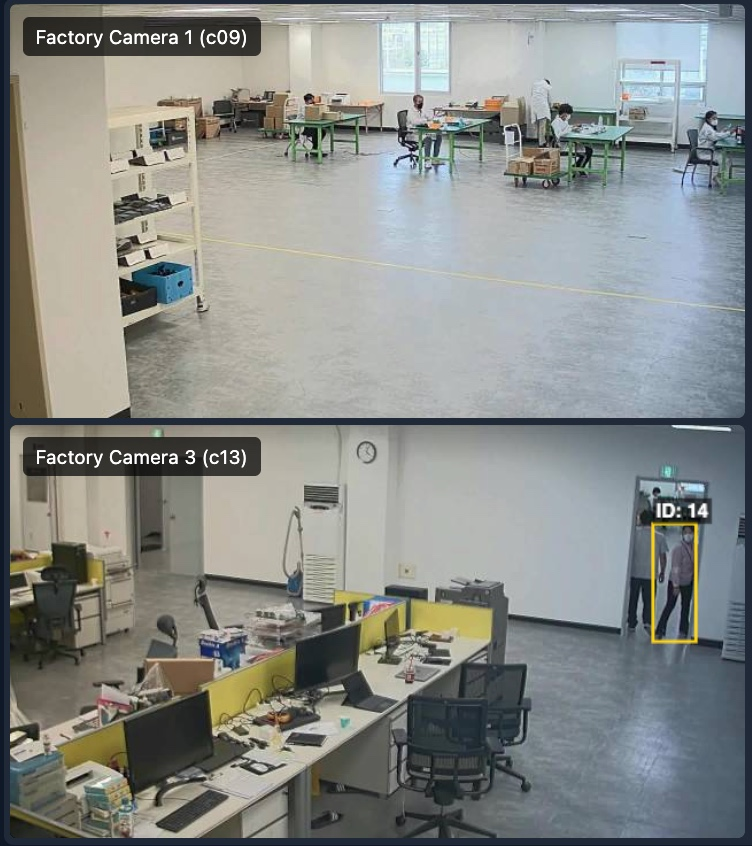
\includegraphics[height=1.1cm]{reid1.jpeg} 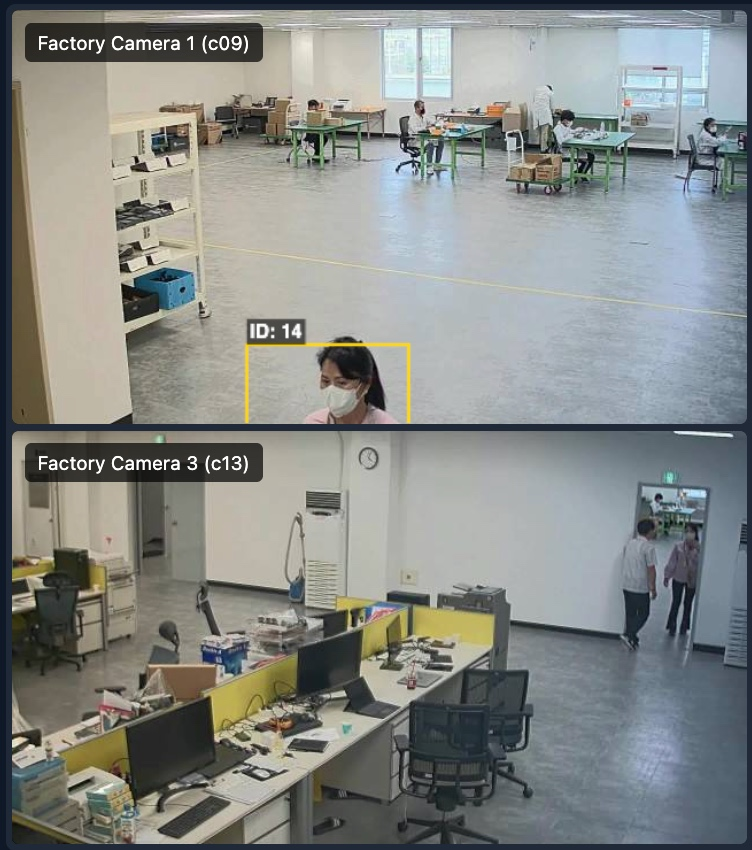
\includegraphics[height=1.1cm]{reid2.jpeg}
};

\draw [arrow] (m4_1) -- (m4_2);
\draw [arrow] (m4_2) -- (m4_3);
\draw [arrow] (m4_3) -- (m4_4);

\begin{scope}[on background layer]
    \node[draw=orange!60, fill=orange!5, mod_container, fit=(m4_1)(m4_4)] (mod4) {};
    \node[modtitle, text=orange!70!black, above=5pt of mod4] {Module 4: Re-ID\\{[}OSNet-AIN{]}};
\end{scope}

\draw [arrow] (dec.south) |- node[below, near start, font=\sffamily\huge\bfseries] {No} (mod4.west);

% ====================
% COLUMN 6: Output
% ====================
\node [output] (out) at ($(mod3.east)!0.5!(mod4.east) + (3.5cm, 0)$) {Global ID Registry\\\&\\2D Floor Plan\\Visualization};

\draw [arrow] (mod3.east) -| (out.north);
\draw [arrow] (mod4.east) -| (out.south);

\end{tikzpicture}
\end{document}
